% Cover letter: Product Manager - AI & 3D, CGTrader (via Talenteek)
% CV: Sections/cv_pm_ai3d.tex -> cv_gen/cv_giovanni_tauro-cgtrader.pdf
\documentclass[11pt,a4paper,sans]{moderncv}
% Shared preamble and header for the cover letters.
% One main file per application: cl_<company>.tex, built to
% cv_gen/coverletter_giovanni_tauro-<company>.pdf next to cv_giovanni_tauro-<company>.pdf.
% Paths (cl_gen/..., Pictures/...) are relative to the project root, as in the CV (see .latexmkrc).

\moderncvstyle{classic}
\moderncvcolor{blue}

\usepackage[scale=0.80]{geometry}
\setlength{\footskip}{136.00005pt}

\usepackage{fontawesome5}
% hyperref is loaded by moderncv itself; loading it here causes an option clash
\usepackage{xcolor}
\usepackage{graphicx}
\ifxetexorluatex
  \usepackage{fontspec}
  \usepackage{unicode-math}
  \defaultfontfeatures{Ligatures=TeX}
  \setmainfont{Latin Modern Roman}
  \setsansfont{Latin Modern Sans}
  \setmonofont{Latin Modern Mono}
  \setmathfont{Latin Modern Math}
\else
  \usepackage[T1]{fontenc}
  \usepackage{lmodern}
\fi

\usepackage[english]{babel}

% used for the PDF title and the letter closing; the visible header is \clheader below
\name{Giovanni}{Tauro}

% Header: #1 = headline under the name (same as the headline of the matching CV)
\newcommand{\clheader}[1]{%
\noindent
\begin{minipage}[c]{0.74\textwidth}
    {\Huge \textbf{Giovanni Tauro}}\\[-0.2em]
    {\small #1}\\[0.3em]

    \footnotesize
    \faMapMarker*~
    \href{https://www.google.com/maps/search/?api=1&query=Lecco+23900+Italy}
    {\color{blue}Bari-Lecco, Italy}
    \quad
    \faPhone*~
    \href{https://wa.me/393279437161}
    {\color{blue}+39 3279437161}
    \quad
    \faEnvelope~
    \href{mailto:giovanni.taurodi@gmail.com}
    {\color{blue}giovanni.taurodi@gmail.com}
    \\[-0.1em]

    \faLinkedin~
    \href{https://www.linkedin.com/in/giovanni-tauro-gt/}
    {\color{blue}LinkedIn}
    \quad
    \faGithub~
    \href{https://github.com/jotades}
    {\color{blue}GitHub}
    \quad
    \faGraduationCap~
    \href{https://scholar.google.com/citations?user=BS0aVGgAAAAJ&hl=it}
    {\color{blue}Scholar}
    \quad
    \faFilePdf~
    \href{https://www.notion.so/Giovanni-Tauro-2a7901d92f3a800b892af425c5875c6a}
    {\color{blue}Portfolio}
    \quad
    \faCubes~
    \href{https://grabcad.com/giovanni.tauro-3}
    {\color{blue}GrabCAD}

\end{minipage}
\hfill
\begin{minipage}[c]{0.18\textwidth}
    \raggedleft
    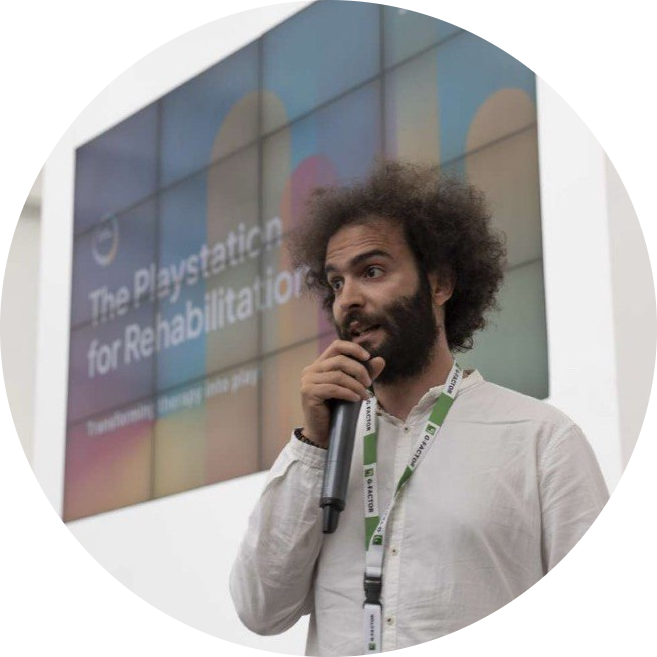
\includegraphics[width=2.8cm]{Pictures/Giovanni_pitch}
\end{minipage}
\vspace{0.1em}
}

\makeatletter
% the sender details are already in \clheader, so skip moderncv's own block
\@detailsfalse
% closing phrase, signature, name
\renewcommand*{\makeletterclosing}{%
  \@closing\\[0.6em]%
  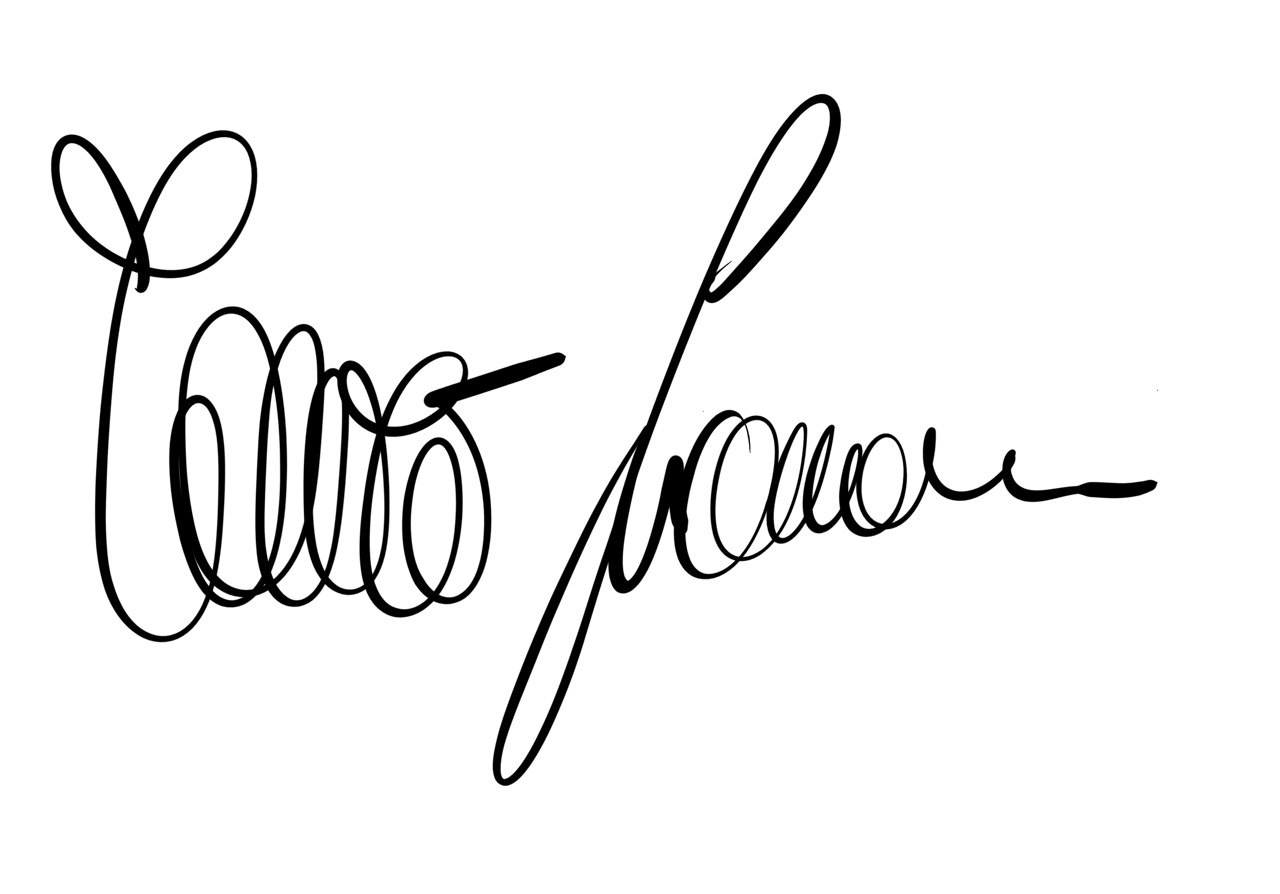
\includegraphics[height=1.2cm]{Pictures/sign_gt.jpg}\\[0.2em]%
  {\bfseries\@firstname~\@lastname}}
\makeatother


\begin{document}

\clheader{Product Manager | AI Prototyping, UX \& 3D}

\recipient{Talenteek}{on behalf of CGTrader}
\opening{Dear Hiring Team,}
\closing{Sincerely,}
\makelettertitle

I am applying for the Product Manager -- AI \& 3D role at CGTrader. I am Head of Product and co-founder of Rehabilia Technologies, and for more than five years I have designed and prototyped products at CNR-STIIMA, the Italian National Research Council. The role asks for someone who takes ideas from ambiguity through prototypes to launch and who uses AI tools every day; that is how I already work, and 3D has been part of my work since my industrial design degree.

At Rehabilia I own the product from discovery to delivery. I interview users and partners, frame the problem, write the requirements and decide what goes into a prototype, an MVP or a later iteration, with a milestone-based roadmap. Our device, PhiCube, reached a usability score of 85.8/100 (SUS) with 19 children and is now in two ongoing multicentre studies with 134 patients. That work taught me to turn a complex system into something its users find simple, and to check it with real people before scaling it.

Claude is part of my everyday work: I use Claude and Claude Code to explore ideas, build coded prototypes and analyse data, and I hold Anthropic's certifications for both. On the 3D side, I have modelled products in SolidWorks and Fusion 360 and built them with 3D printing and 3D scanning, and at CNR-STIIMA I created and optimised Blender and Unity assets for a driving simulator, published at ICCHP 2022 (\href{https://link.springer.com/chapter/10.1007/978-3-031-08645-8_56}{\color{blue}Springer}), and a VR wheelchair simulator. So I know first-hand where 3D workflows are slow (modelling, cleanup, texturing, optimisation, preparing a file for print) and where generative AI could help.

I have not yet worked on a marketplace or a consumer creative tool, and my users so far have been clinicians, researchers and partners. What I bring is the habit of learning a new domain from its users, prototyping quickly and deciding with evidence what to build next. My portfolio and GrabCAD models are linked above.

I would welcome the chance to discuss the role further.

\makeletterclosing

\end{document}
